\documentclass[a4paper,10pt]{article}
\usepackage[utf8x]{inputenc}
\usepackage[serbian]{babel}

\usepackage[version=3]{mhchem} % Package for chemical equation typesetting
\usepackage[margin=2.5cm]{geometry}
\usepackage{siunitx} % Provides the \SI{}{} and \si{} command for typesetting SI units
\usepackage{graphicx} % Required for the inclusion of images
\usepackage{natbib} % Required to change bibliography style to APA
\usepackage{amsmath} % Required for some math elements 
\usepackage{subfig} % For multiple figures side-by-side
\usepackage{url} % For linking url's properly

\setlength\parindent{0pt} % Removes all indentation from paragraphs

%\usepackage{times} % Uncomment to use the Times New Roman font

%----------------------------------------------------------------------------------------
%	DOCUMENT INFORMATION
%----------------------------------------------------------------------------------------

\title{OPNA: Drugi projektni zadatak \\ Šturmova teorema} % Title

\author{Aleksa \textsc{Ilić}} % Author name

\date{\today} % Date for the report

\begin{document}

\maketitle % Insert the title, author and date

\begin{abstract}
    Rad prikazuje praktičnu realizaciju konzolnog programa koji izvršava numeričku procenu Šturmove teoreme sa arbitrarnom preciznošću i modularnošću ispisa
\end{abstract}

%----------------------------------------------------------------------------------------
%	SECTION: UVOD
%----------------------------------------------------------------------------------------

\section{Uvod}
\subsection{Opis problema}

Opis problema ovde

\begin{itemize}
\item Item 1
\end{itemize}

Zadatak ovde

\subsection{Definicije}
\label{definitions}
\begin{description}
\item[Pojam 1] Opis pojma
\end{description}
Date definicije preuzete iz rada RAD OVDE.
 
%----------------------------------------------------------------------------------------
%	SECTION: OPIS REŠENJA
%----------------------------------------------------------------------------------------

\section{Opis rešenja}

Za realizaciju rešenja korišćen je programski jezik \textbf{C++17} zajedno sa najnovijom verzijom \textbf{Boost} biblioteka u trenutku pisanja ovog rada. Celokupan, dokumentovani izvorni kod dostupan je na autorovom github profilu \cite{WEBSITE:Github}.

Dalji opis resenja ovde

\begin{figure}
\begin{center}
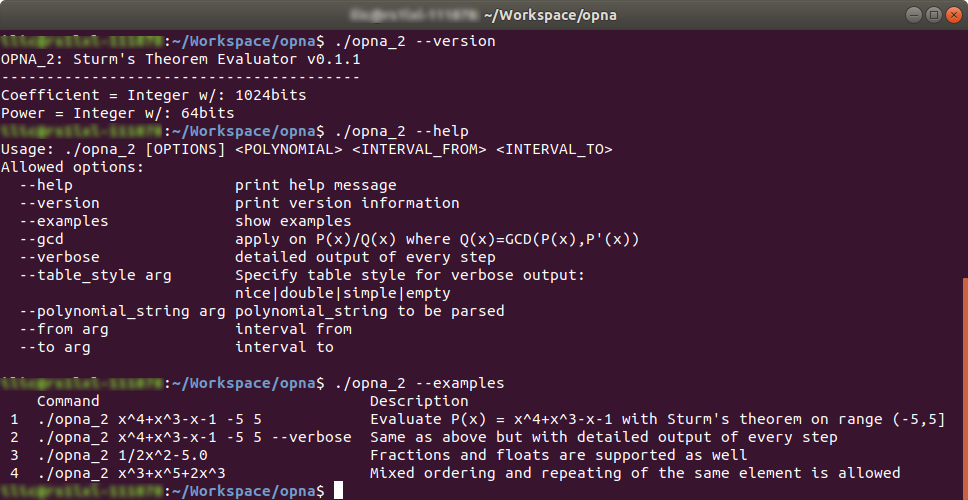
\includegraphics[width=0.9\textwidth]{version.png}
\caption{Podrazumevana podešavanja i pomoćni ekran}
\label{fig:version}
\end{center}
\end{figure}

\subsection{Primeri ispisa}

Par primera ispisa ovde

\newpage

%----------------------------------------------------------------------------------------
%	SECTION: RAČUN
%----------------------------------------------------------------------------------------

\section{Izračunavanje \textit{tog i tog polinoma}}
Definicija problema

\subsection{Podešavanja programa}
Za prikaz rešenja korišćene su podrazumevane veličine tipova, itd.

\subsection{Rezultati}

\begin{verbatim}
Output programa ovde 
\end{verbatim}

%----------------------------------------------------------------------------------------
%	SECTION: DISKUSIJA
%----------------------------------------------------------------------------------------

\section{Diskusija rezultata}

Diskusija rezultata ovde

%----------------------------------------------------------------------------------------
%	BIBLIOGRAPHY
%----------------------------------------------------------------------------------------

\bibliographystyle{apalike}

\bibliography{sample}

%----------------------------------------------------------------------------------------


\end{document}
